\chapter{Logistic Regression}

Now we turn away from regression to classification problems. Don't be confused by the name `logistic regression,' it's actually just named for the mathematical function and it's a common approach to classification.

\section{Binary Classification}
In classification problems, instead of our output being continuous, we expect it to fall into discrete classes. We'll start with the simplest case: binary classification. Here, we have our output variable $y \in \{0, 1\}$. Typically, we take $0$ as the negative class and $1$ as the positive class. 

Consider the following example: we have a sample of eight tumors, and we want to determine if they're malignant based on the tumor size. These are plotted in Figure \ref{logreg-eg-maltumor-noregline}. One thing we can do is assume a linear relationship with hypothesis $h_\theta\left( \vec{x} \right) = \vec{\theta}^\intercal \vec{x}$. This shown in Figure \ref{logreg_eg1_maltumor_linreg1}.

\begin{figure}[h]
	\centering
	\begin{subfigure}[t]{0.45\textwidth}
   		\centering
    		\graphicspath{{./Figures/}}
  		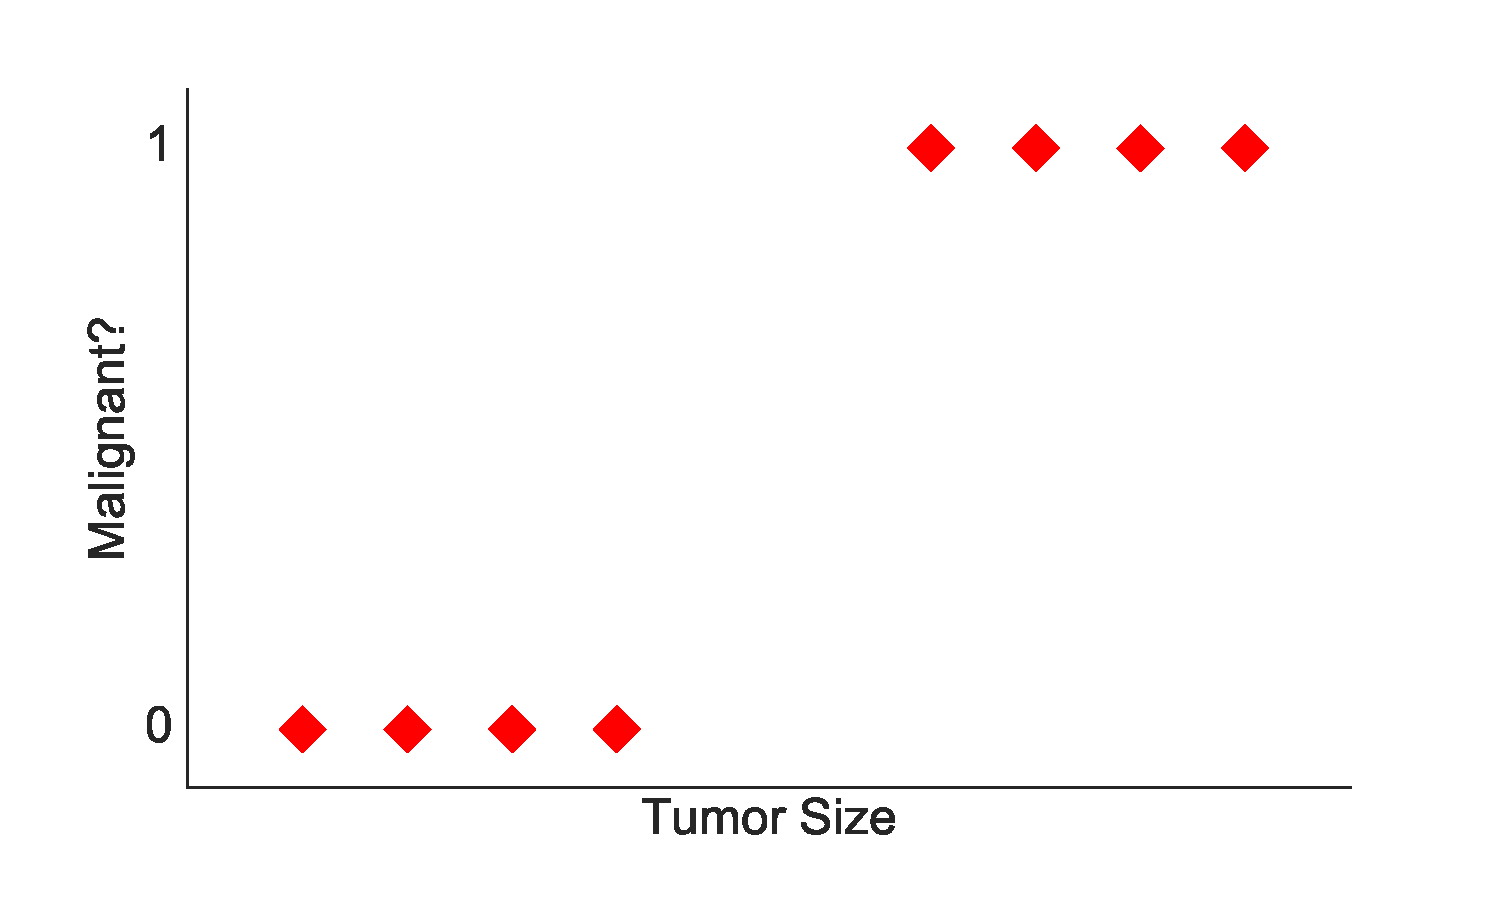
\includegraphics[scale=0.3]{logreg_eg1_maltumor.pdf} 
   		\caption[]{Plot of tumors by size. }
   		\label{logreg-eg-maltumor-noregline}
	\end{subfigure}
	\begin{subfigure}[t]{0.45\textwidth}
   		\centering
    		\graphicspath{{./Figures/}}
   		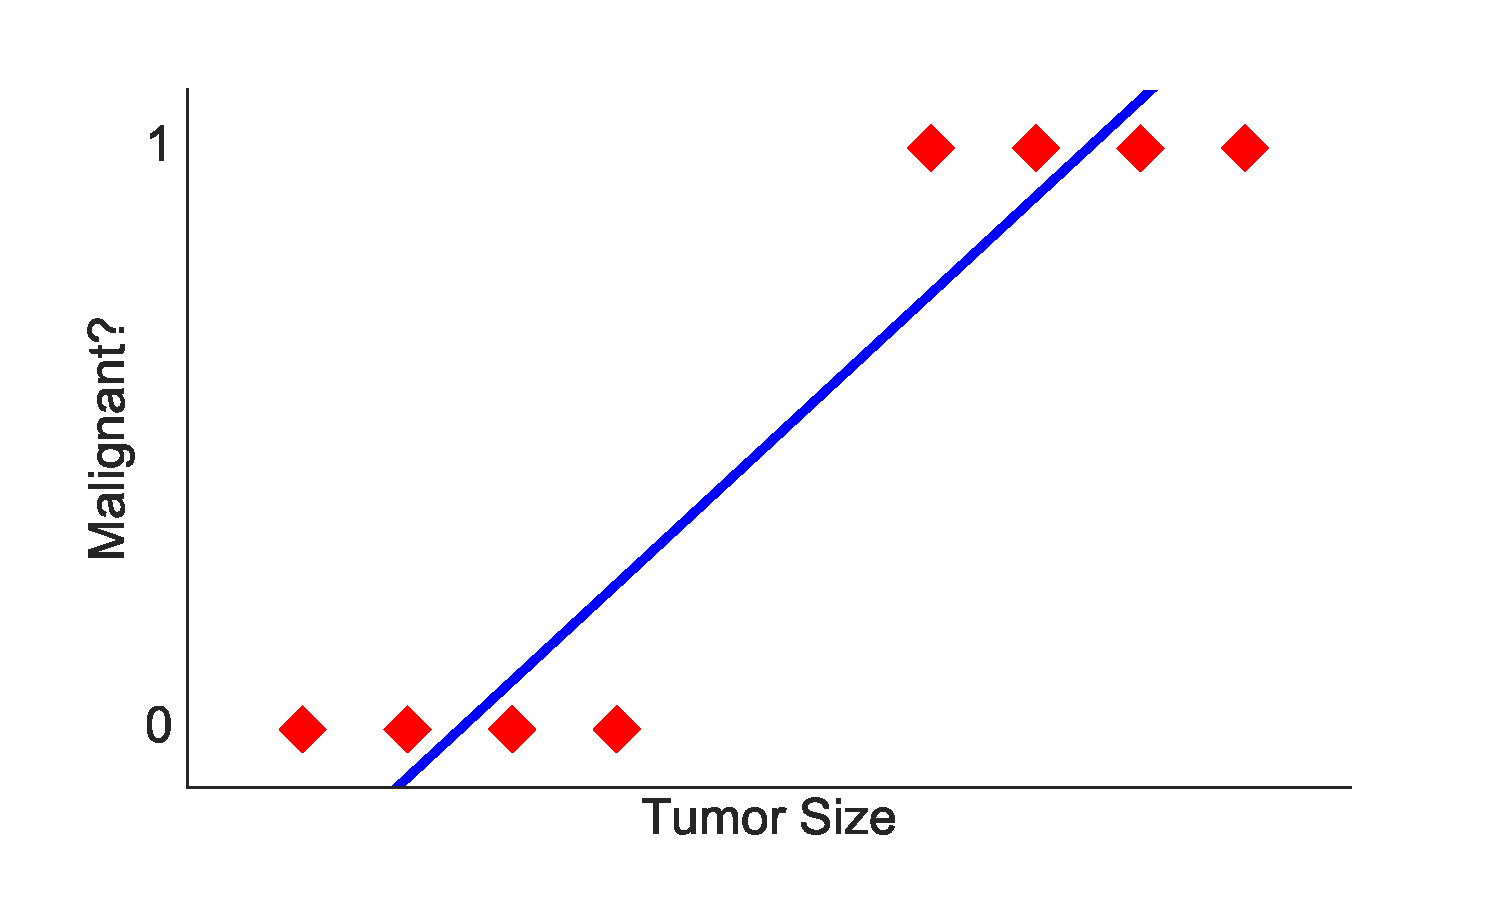
\includegraphics[scale=0.3]{logreg_eg1_maltumor_linreg1.pdf} 
   		\caption[]{Plot of tumors by size with linear regression line $y =  \frac{x-1}{6} - 0.25$.}
   		\label{logreg_eg1_maltumor_linreg1}
	\end{subfigure}
\end{figure}

To try and make predictions, we can threshold the output at $h_\theta\left( x \right) = 0.5$, and then:
\begin{itemize}
\item If $h_\theta\left(x\right) \geq 0.5$, then predict $y = 1$
\item If $h_\theta\left( x \right) < 0.5$, then predict $y = 0$
\end{itemize}
and you can see this in Figure \ref{logreg_eg1_maltumor_linreg1_threshold.pdf}.

\begin{figure}[h] 
	\centering
	\graphicspath{{./Figures/}} 
	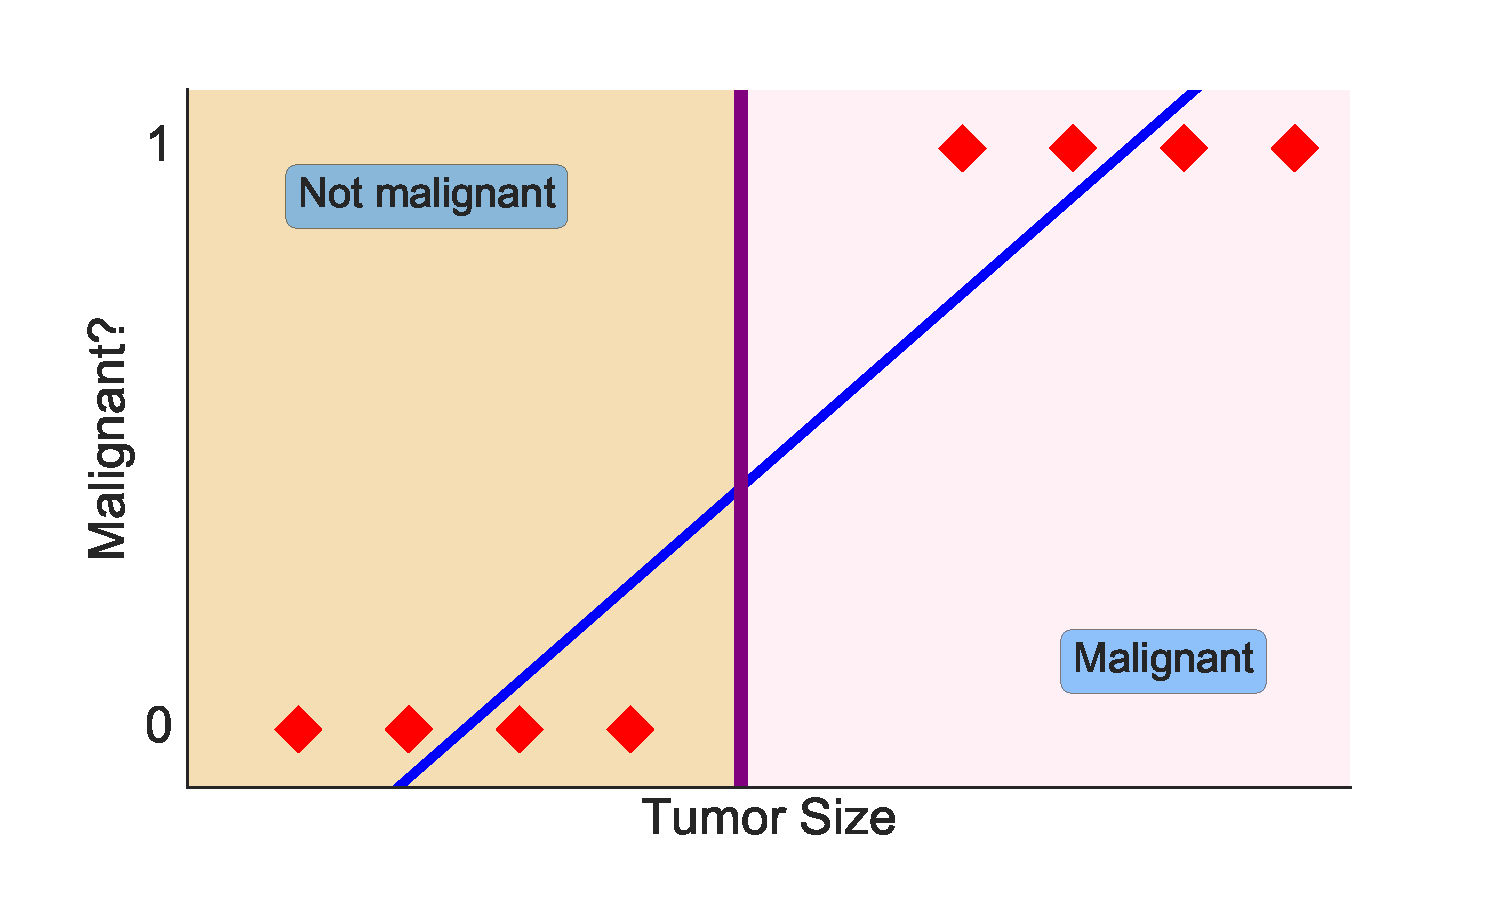
\includegraphics[scale=0.4]{logreg_eg1_maltumor_linreg1_threshold.pdf} 
	\caption[]{Linear regression plotted with classification regions. }
	\label{logreg_eg1_maltumor_linreg1_threshold.pdf}
\end{figure}


In this example, it would seem like linear regression is a good classifier. However, what if we add a new data point for a large tumor. Suddenly, our results look like this

\begin{figure}[h] %  figure placement: here, top, bottom, or page
	\centering
	\graphicspath{{./Figures/}} %Use this to import an image from a subfolder.
	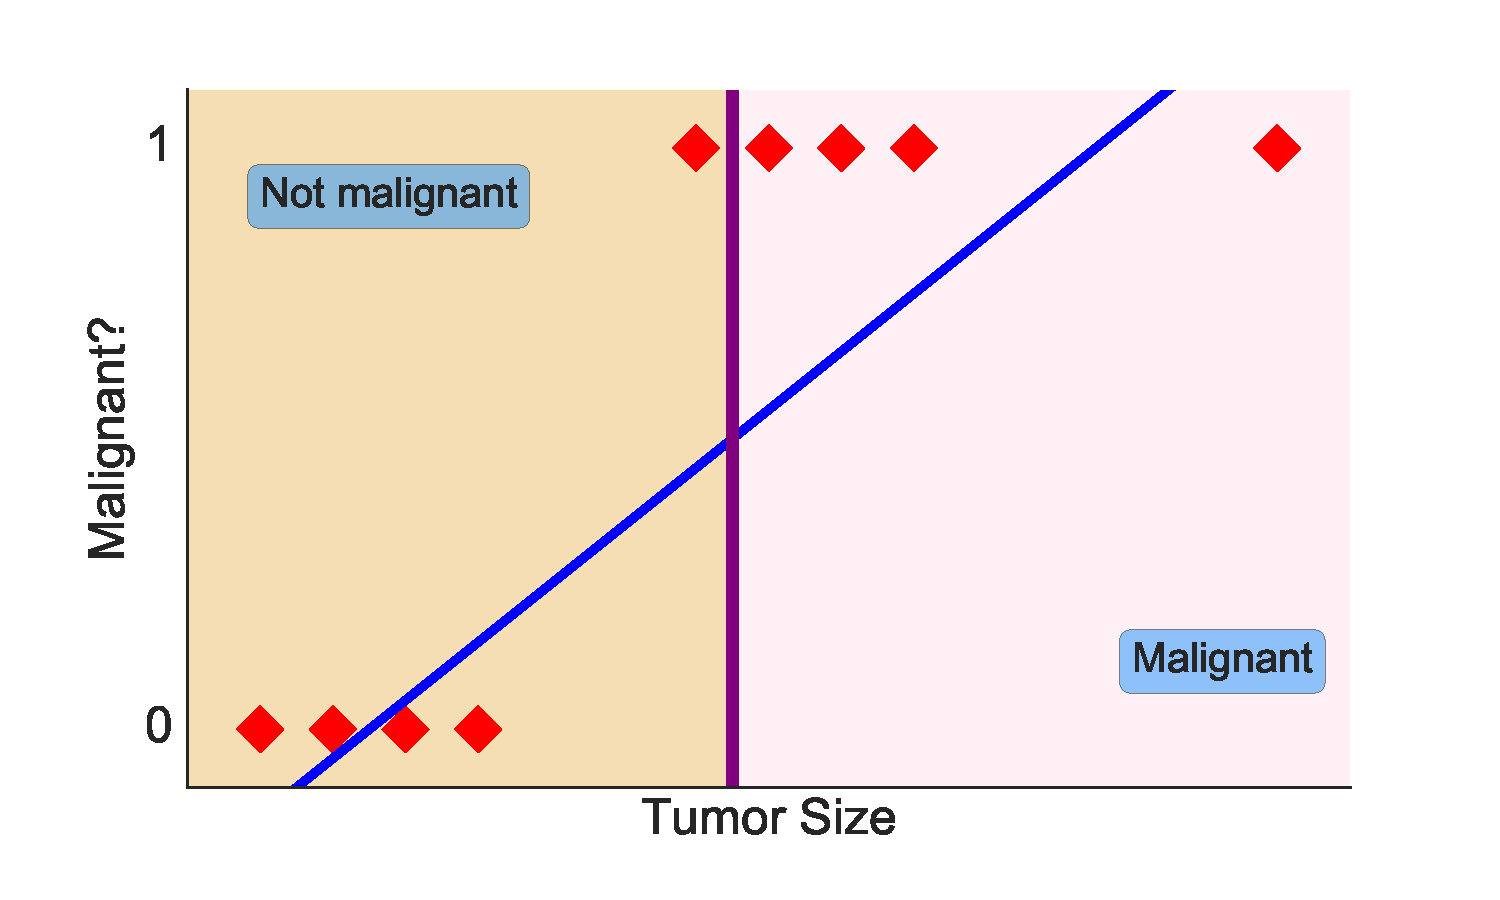
\includegraphics[scale=0.4]{logreg_eg1_maltumor_linreg1_newpoint.pdf} 
	\caption[]{Linear regression plotted with classification regions after a new data point is added. Notice how one of the malignant tumors is now being misclassified as benign.}
	\label{logreg_eg1_maltumor_linreg1_newpoint.pdf}
\end{figure}

and now, we have a malignant tumor being misclassified as benign. Ergo, maybe linear regression isn't the best way to build a binary classifier. 






\section{Hypothesis Representation}
In linear regression, our hypothesis was $h_\theta\left(\vec{x}\right) = \vec{\theta}^\intercal \vec{x}$ For logistic regression, we want our hypothesis to satisfy $0 \leq h_\theta\left(x\right) \leq 1$. To do this, we use the sigmoid function.\footnote{This is also called the logistic function, and is the namesake for logistic regression.} To make this work, we modify our hypothesis to be
\begin{equation}
h_\theta\left(x\right) = g\left(\vec{\theta}^\intercal \vec{x}\right)
\end{equation}
where the function $g\left(z\right)$ is defined as
\begin{equation}
g\left(z\right) = \frac{1}{1 + e^{-z}}
\end{equation}
Thus, to get the hypothesis function using the sigmoid function, just set $z = \vec{\theta}^\intercal \vec{x}$. 

The sigmoid function, shown in Figure \ref{logreg_eg2_sigmoid_func_plot.pdf}, maps any real number onto the interval $\left(0, 1\right)$. This makes it immensely useful for transforming an arbitrary function for use with classification.


\begin{figure}[h] %  figure placement: here, top, bottom, or page
	\centering
	\graphicspath{{./Figures/}} %Use this to import an image from a subfolder.
	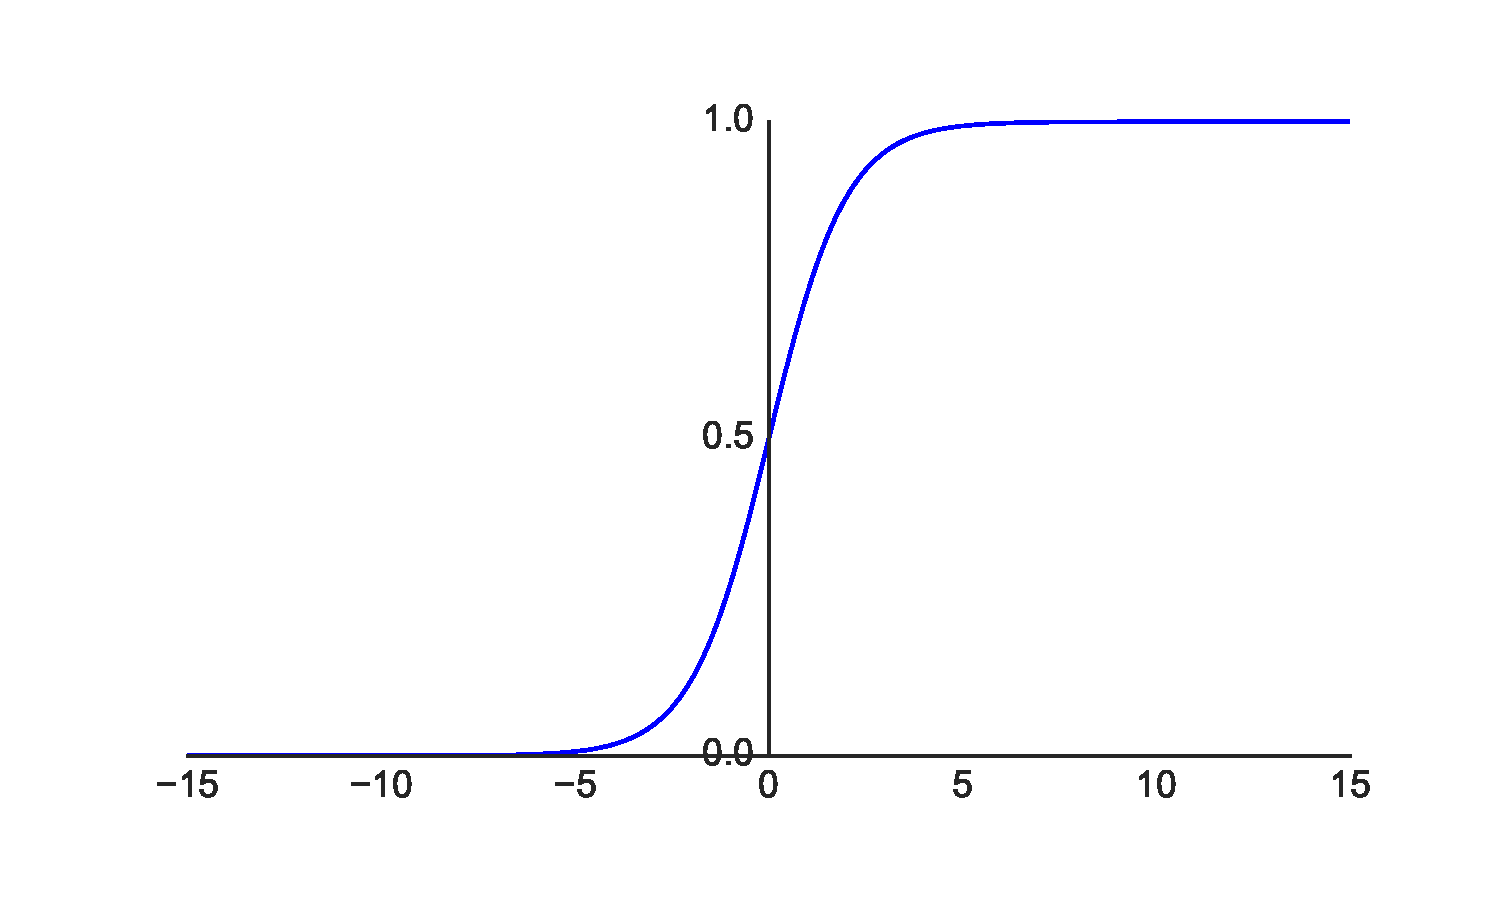
\includegraphics[scale=0.4]{logreg_eg2_sigmoid_func_plot.pdf} 
	\caption[]{Sample plot of the sigmoid function.}
	\label{logreg_eg2_sigmoid_func_plot.pdf}
\end{figure}


\subsection{Interpretation of the Logistic Hypothesis Function}

When examining the hypothesis function output for logistic regression, we interpret $h_\theta\left(x \right)$ is the estimated probability that $y=1$ on an input example $x$. For example, let's revisit the tumor size question from above. We have 
$$
\vec{x} = \left[\begin{array}{c}x_0 \\ x_1 \end{array}\right] = \left[\begin{array}{c}1 \\ \text{tumor size} \end{array}\right]
$$
If our hypothesis $h_\theta\left( x \right) = 0.7$, then we can tell the patient that there is a 70\% chance of the tumor being malignant. 

Slightly more formally, we interpret $h_\theta\left(x\right)$ as:\footnote{This is read as "the probability that $y = 1$, given $x$, parameterized by $\theta$.}
\begin{equation}
h_\theta\left(x\right) = P\left(y=1 | x; \theta\right)
\end{equation}
Thus, by the rules of probability:
\begin{align}
P\left(y=0 | x; \theta\right) + P\left(y=1 | x; \theta\right) = 1 \\
P\left(y=0 | x; \theta\right) = 1 - P\left(y=1 | x; \theta\right)
\end{align}

\section{Decision Boundary}








































